\documentclass[12pt]{article}
\usepackage[top=1in, bottom=1in, left=1in, right=1in]{geometry}
%\usepackage[margin=1in]{geometry}
\usepackage[onehalfspacing]{setspace}
%\usepackage[doublespacing]{setspace}
\usepackage{amsmath, amssymb, amsthm}
\usepackage{enumerate, enumitem}
\usepackage{fancyhdr, graphicx, proof, comment, multicol}
%\usepackage[none]{hyphenat} % This command prevents hyphenation of words
\binoppenalty=\maxdimen % This command and the next prevent in-line equation breaks
\relpenalty=\maxdimen
%    Good website with common symbols
% http://www.artofproblemsolving.com/wiki/index.php/LaTeX%3ASymbols
%    How to change enumeration using enumitem package
% http://tex.stackexchange.com/questions/129951/enumerate-tag-using-the-alphabet-instead-of-numbers
%    Quick post on headers
% http://timmurphy.org/2010/08/07/headers-and-footers-in-latex-using-fancyhdr/
%    Info on alignat
% http://tex.stackexchange.com/questions/229799/align-words-next-to-the-numbering
% http://tex.stackexchange.com/questions/43102/how-to-subtract-two-equations
%    Text align left-center-right
% http://tex.stackexchange.com/questions/55472/how-to-make-text-aligned-left-center-right-in-the-same-line
\usepackage{microtype} % Modifies spacing between letters and words
\usepackage{mathpazo} % Modifies font. Optional package.
\usepackage{mdframed} % Required for boxed problems.
\usepackage{parskip} % Left justifies new paragraphs.
\linespread{1.1} 


%figure support
\usepackage{import}
\usepackage{xifthen}
\pdfminorversion=7
\usepackage{pdfpages}
\usepackage{transparent}
\newcommand{\incfig}[1]{%
	\def\svgwidth{\columnwidth}
	\import{./figures/}{#1.pdf_tex}
}
\graphicspath{ {./figures/} }
\pdfsuppresswarningpagegroup=1


\newenvironment{problem}[1]
{\begin{mdframed}[linewidth=0.6pt]
        \textsc{Problem #1:}

}
    {\end{mdframed}}

\newenvironment{solution}
    {\textsc{Solution:}\\}
    {\newpage}% puts a new page after the solution

\newenvironment{statement}[1]
{\begin{mdframed}[linewidth=0.6pt]
        \textsc{Statement #1:}

}
    {\end{mdframed}}

%\newenvironment{prf}
 %   {\textsc{Proof:}\}
 %   {\newpage}% puts a new page after the solution

\newcommand{\R}{\mathbb{R}}
\newcommand{\C}{\mathbb{C}}
\newcommand{\Z}{\mathbb{Z}}
\newcommand{\N}{\mathbb{N}}
\newcommand{\Q}{\mathbb{Q}}

\begin{document}
% This is the Header
% Make sure you update this information!!!!
\noindent
\textbf{CIS 4367.01} \hfill \textbf{Brandon Thompson} \\
\normalsize Prof. Elibol \hfill Due Date: 1/15/20 \\

% This is where you name your homework
\begin{center}
\textbf{Homework 1}
\end{center}
	\begin{problem}{\#1.1}
		Consider an automated teller machine (ATM) in which users provide a personal
		identification number (PIN) and a card for account access. Give examples of
		confidentiality, integrity, and availability requirements
		associated with the system and, in each case indicate the degree of importance
		of the requirement.
	\end{problem}
	\begin{solution}
		\textbf{Confidentiality:} System must keep personal information private
		in the system and during transmission. If an attacker gains access
		to someones PIN number they could gain access to their account.\\
		\textbf{Integrity:} Financial data can only be modified by supplying funds
		from another account or cash (withdraw or deposit). Editing financial
		information could be catastrophic for the bank, allowing an attacker to
		withdraw an infinite amount of funds.\\
		\textbf{Availability:} Availability of the host is important, but
		individual teller machines is less so.
	\end{solution}

	\begin{problem}{\#1.2}
		Repeat Problem 1.1 for a telephone switching system that routes calls through a
		switching network based on the telephone number requested by the caller.
	\end{problem}
	\begin{solution}
		\textbf{Confidentiality:} Company keeps call logs but
		users may not want others to know who they are calling however it is not 
		crucial to keep private. Low security should be enough.\\
		\textbf{Integrity:} Users should be assured that the number they are calling
		is actually routing to the correct number.\\
		\textbf{Availability:} System should be available whenever someone tries
		to call a number.
	\end{solution}

	\begin{problem}{\#1.3}
		Consider a desktop publishing system used to produce documents for various
		organizations.
		\begin{enumerate}[label=\alph*]
			\item Give an example of a type of publication for which confidentiality
				of the stored data is the most important requirement.
			\item Give an example of a type of publication in which data integrity
				is the most important requirement.
			\item Give an example in which system availability is the most important
				requirement.
		\end{enumerate}
	\end{problem}
	\begin{solution}
		\begin{enumerate}[label=\alph*]
			\item If system is publishing corporate proprietary information, the
				company will not want anyone else to have access to the
				documents.
			\item Laws and regulations need be be assured that they are valid
				and have not been tamped with.
			\item If system is publishing news then is should be available any time.
		\end{enumerate}
	\end{solution}

	\begin{problem}{\#1.4}
		For each of the following assets, assign a low, moderate, or high impact level
		for the loss of confidentiality, availability and integrity respectively.
		Justify your answers.
		\begin{enumerate}[label=\alph*]
			\item An organization managing public information on its Web server.
			\item A law enforcement organization managing extremely sensitive
				information.
			\item A financial organization managing routine administrative
				information (non privacy-related information).
			\item An information system used for large acquisitions in a contracting
				organization contains both sensitive, pre-solicitation phase
				contract information and routine administrative information.
				Assess the impact for the two data sets separately and the 
				information system as a whole.
			\item A power plant contains a SCADA (supervisory control and data
				acquisition) system controlling the distribution of electric
				power for a large military installation. The SCADA system
				contains both real-time sensor data and routine administrative
				information. Assess the impact for the two data sets separately
				and the information system as a whole.
		\end{enumerate}
	\end{problem}
	\begin{solution}
		\begin{enumerate}[label=\alph*]
			\item \textbf{Confidentiality:} Low, information is already public.\\
				\textbf{Integrity:} Medium, if many people are looking at this
				information is should be correct. But it would not catastrophic if
				information was changed.\\
				\textbf{Availability:} Medium, if a lot of people are using this
				web server, then it should be available as much as possible.
			\item \textbf{Confidentiality:} High, extremely sensitive data should
				only be able to be viewed by authorized users.\\
				\textbf{Integrity:} High, if data was lost or modified it could
				impact investigations.\\
				\textbf{Availability:} Medium, if system is unavailable, users
				would be unable to work.
			\item \textbf{Confidentiality:} Low, routine administrative information
				does not need a lot of protection.\\
				\textbf{Integrity:} Medium, would not be a huge deal if this information
				was corrupted.\\
				\textbf{Availability:} High, if the data is used frequently, then
				having it available when necessary is important.
			\item \textbf{Confidentiality:} Pre-solicitation data should be high priority level
				routine data less so.\\
				\textbf{Integrity:} Pre-solicitation data should be medium as well
				as routine administrative data and the entire system,\\
				\textbf{Availability:} Pre-solicitation data low, routine data medium,
				whole system medium.
			\item \textbf{Confidentiality:} Real-time data would not seem important to
				keep confidential, low, administrative data, medium, system medium.\\
				\textbf{Integrity:} Modifying real-time data could lead to power failures
				throughout the military installation, high. Administrative data
				should be medium.\\
				\textbf{Availability:} Real-time data should be available at all times
				by the SCADA system, or there could be power outages, high.
				Routine administrative data should be medium if the data is used
				often.
		\end{enumerate}
	\end{solution}

	\begin{problem}{\#1.5}
		Consider the following general code for allowing access to a resource:
		\begin{verbatim}
			DWORD dwRet = isAccessAllowed(...);
			if (dwRet == ERROR_ACCESS_DENIED) {
			// Security check failed.
			// Inform user that access is denied.
			} else {
			// Security check OK.
		    	}
		\end{verbatim}
		\begin{enumerate}[label=\alph*]
			\item Explain the security flaw in this program.
			\item Rewrite the code to avoid this flaw.\\
				\textit{Hint:} Consider the design principal of fail-safe defaults.
		\end{enumerate}
	\end{problem}
	\begin{solution}
		\begin{enumerate}[label=\alph*]
			\item The security flaw in this code comes from if the \verb|isAccessAllowed()|
				function is unable to execute properly. Security check needs to proceed
				if there are no errors, not if it is equal to a single error.
			\item
				\begin{verbatim}
					DWORD dwRet = isAccessAllowed(...);
					if (dwRet == NO_ERROR) {
					    //Secure check OK.
					    //Perform task.
					} else {
					    //Security check failed.
					    //Inform user that access is denied.
					}
				\end{verbatim}
		\end{enumerate}
	\end{solution}

	\begin{problem}{\#1.6}
		Develop and attack tree for gaining access to the contents of a physical safe.
	\end{problem}
	\begin{solution}
		\begin{figure}[ht!]
			\centering
			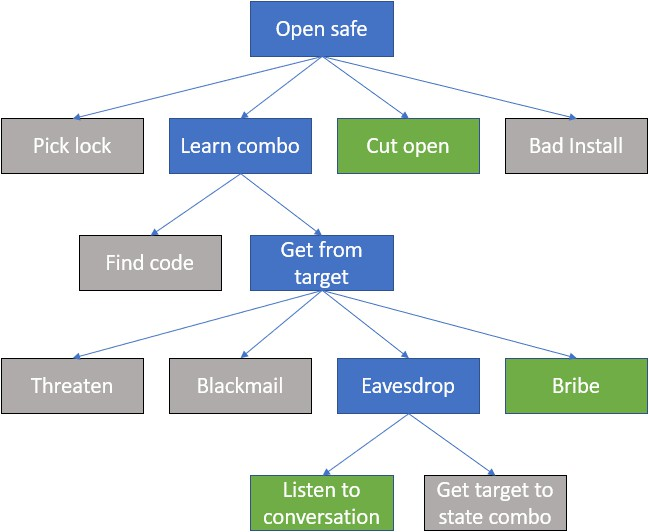
\includegraphics[width=0.8\textwidth]{comp_sec_hw1_q6}
		\end{figure}
	\end{solution}
\end{document}
